% ~ 12 pages
\chapter{Identification of Hadronic Tau Lepton Decays using Boosted Decision
  Trees}
\label{sec:bdt}
The reconstruction of hadronic tau lepton decays described in
Chapter~\ref{sec:reconstruction} is based on jets reconstructed using the
anti-$k_\text{t}$ jet algorithm operating on clusters of calorimeter cells. Jets
originating from quarks or gluons, which are more abundant than tau leptons due
to the large multijet production cross section at the LHC, are often
reconstructed as candidates for hadronic tau lepton decays and represent a
significant background in many analyses. The reconstruction itself offers little
rejection of \tauhadvis candidates from quark- or gluon-initiated jets with the
exception of the track classification when requiring 1- or 3-track decays. In
the ATLAS experiment an identification algorithm based on multivariate methods
utilising track and shower shape variables is used to discriminate hadronic tau
decays from \tauhadvis reconstructed in multijet events.

This chapter will start with a description of the tau identification procedure
including definitions of the discriminating variables and the configuration of
the BDTs used for distinguishing \tauhadvis from hadronic tau decays (signal
candidates) and \tauhadvis originating from quark- or gluon-initiated jets
(background candidates). The simulated event samples used for training and
performance evaluation of the models, the kinematic reweighting and the
preselection will be described. Subsequently, a systematic optimisation of the
BDT is performed to improve the discriminative power of the tau identification.
For this the configuration of the BDT and the variable selection is
investigated. The chapter is concluded by evaluation the performance of the
optimised BDTs.

In the following two figures of merit will be used to describe the performance
of the tau identification. They are based on the definition of the efficiency of
a selection given by:
\begin{align*}
  \text{Efficiency} = \frac{\text{Number of reconstructed \tauhadvis passing a selection}}{\text{Total number of reconstructed \tauhadvis}} \eqdot
\end{align*}
Notably the efficiencies given in this chapter will not account for
inefficiencies in the reconstruction. The signal efficiency is the efficiency of
selecting \tauhadvis candidates in a signal sample with candidates originating
from hadronic tau lepton decays. The background rejection is the inverse
efficiency of selecting \tauhadvis in a background sample containing fake
\tauhadvis candidates. Hereafter, the signal efficiency and background rejection
will be referred to as efficiency and rejection, respectively. The aim of this
chapter is to improve the rejection of \tauhadvis originating from quark- or
gluon-initiated jets at a fixed signal efficiency such that analyses using tau
identification observe higher signal significances due to a larger
signal-to-background ratio.

\section{Description of the Tau Identification Procedure}
\label{sec:bdt_tauid}
The tau identification algorithm currently in use in the ATLAS experiment
employs BDTs with high-level input variables. The identification uses separate
BDTs for the 1- and 3-prong identification with different sets of input
variables. Classification with BDTs return a score measuring the confidence of
the binary decision. This allows a trade-off between signal efficiency and
background rejection by choosing different decision thresholds. In the ATLAS
experiment these thresholds are parametrised as functions of the reconstructed
visible transverse momentum~$p_\text{T}$ of the \tauhadvis at tau energy scale
and the average number of interactions per bunch crossing~$\mu$ such that the
signal efficiency is constant in different momentum and pile-up regimes.

\subsection{Discriminating Variables}
\label{sec:bdt_features}

Photons originating from neutral pions in hadronic tau lepton decays typically
deposit their energy in the Presampler and first two layers of the
electromagnetic calorimeter and energy depositions in EM3 generally originate
from charged hadrons produced in the tau decay. Therefore, the third layer of
the electromagnetic calorimeter is considered to be part of the hadronic
calorimeter when defining the identification variables.

The variables defined in Ref.~\cite{atlas:taurec:run2} are updated to contain
the latest changes in the reconstruction, the largest being the introduction of
the multivariate track classification algorithm. They target the features of
hadronic tau decays discussed in Section~\ref{sec:features_tau_decay}. The
definitions are:
\begin{description}
\item[Central energy fraction ($f_\text{cent}$):] Fraction of transverse energy
  at EM scale deposited in calorimeter cells with a barycentre in a cone of
  radius $\Delta R < 0.1$, and cells in a cone of radius $\Delta R < 0.2$ with
  respect to the reconstructed tau axis.
  % (i.e.\ the axis after correcting for the position of the primary vertex cf.\
  % section~\ref{sec:reco_vertex_assoc}).
  For noise suppression the calorimeter cells must be part of a
  \emph{TopoCluster}.

\item[Inverse momentum fraction of the leading track
  ($f_\text{leadtrack}^{-1}$):] Fraction of transverse energy at EM scale
  deposited in calorimeter cells (as part of \emph{TopoClusters}) with a
  barycentre in a cone of radius~$\Delta R < 0.2$ with respect to the tau axis
  and the transverse momentum of the highest transverse momentum track
  classified as \emph{charged} according to the track classification.

\item[Track radius ($R_\text{track}$):] Mean $\Delta R$-distance of tracks
  classified as \emph{charged} and the tau axis weighted by the transverse
  momentum of each track.

\item[Maximum track $\Delta R$ ($\Delta R_\text{max}$):] Maximum
  $\Delta R$-distance of all tracks classified as \emph{charged} with respect to
  the tau axis. Equivalent to $R_\text{track}$ for 1-track \tauhadvis.

\item[Transverse impact parameter significance of the leading track
  ($| S_\text{leadtrack} |$):] Absolute value of the transverse impact
  parameter~$d_0$ of the leading \emph{charged} track with respect to the
  reconstructed primary vertex divided by its uncertainty estimate from the
  track and vertex fit.

\item[Transverse flight path significance ($S_\text{T}^\text{flight}$):]
  Distance between the secondary vertex reconstructed using tracks classified as
  \emph{charged} and primary vertex in the transverse plane divided by the
  estimated uncertainty from the secondary vertex fit.

\item[Momentum fraction of isolation tracks ($f_\text{iso}^\text{track}$):] Sum
  of transverse momenta of \emph{modified isolation} tracks divided by the sum
  of transverse momenta of \emph{modified isolation} and \emph{charged} tracks.

\item[EM energy fraction of charged pions ($f_\text{EM}^\text{track-HAD}$):]
  Energy deposited by charged pions in the electromagnetic part of the
  calorimeter estimated by subtracting the energy contained in the hadronic part
  of \emph{TopoClusters} from the energy of the track system, consisting of
  tracks classified as \emph{charged}, estimated by the scalar sum of track
  momenta. This energy is divided by the energy contained in the electromagnetic
  part of clusters associated with the jet seeding the \tauhadvis. All cluster
  energies are calibrated at LC scale.

\item[Ratio of EM energy and track momentum ($f_\text{track}^\text{EM}$):]
  Energy deposited as part of \emph{TopoClusters} of the reconstructed jet in
  the electromagnetic part of the calorimeter calibrated at LC scale, divided by
  the scalar momentum sum of tracks classified as \emph{charged}.

\item[Fraction of track-plus-EM-system $p_\text{T}$
  ($p_\text{T}^\text{EM+track} / p_\text{T}$):] Transverse momentum of the
  visible tau decay estimated from the four-momentum sum of \emph{charged}
  tracks (assuming $\pi^\pm$ mass) and up to two of the most-energetic clusters
  (assuming zero mass) in the electromagnetic part of the calorimeter, divided
  by the visible transverse momentum of the \tauhadvis at LC scale.

\item[Mass of the track-plus-EM-system ($m_\text{EM+track}$):] Invariant mass of
  the visible tau decay estimated from the four-momentum sum of \emph{charged}
  tracks (assuming $\pi^\pm$ mass) and up to two of the most-energetic clusters
  (assuming zero mass) in the electromagnetic part of the calorimeter.

\item[Mass of the track system ($m_\text{track}$):] Invariant mass of the system
  consisting of tracks classified as \emph{charged} using a $\pi^\pm$ mass
  hypothesis.
\end{description}
An example of two important variables for identifying hadronic tau lepton decays
is depicted in Figure~\ref{fig:bdt_discriminants}. The remaining variables are
omitted for brevity and can be found in Appendix~\ref{app:tauid_vars}. The
momentum fraction of isolation tracks~\smash{$f_\text{iso}^\text{track}$} in
1-prong \tauhadvis candidates shows that isolation tracks often carry a large
momentum fraction for background candidates, while signal candidates often do
not have reconstructed isolation tracks. Moreover, the invariant mass of the
track system for 3-prong \tauhadvis candidates shows a peak for signal
candidates below the mass of the tau lepton, while background candidates can
have large invariant masses. Table~\ref{tab:baseline_variables} summarises the
variable selection for the 1- and 3-prong BDTs.

\begin{figure}[htb]
  \begin{subfigure}[t]{0.48\textwidth}
    \centering
    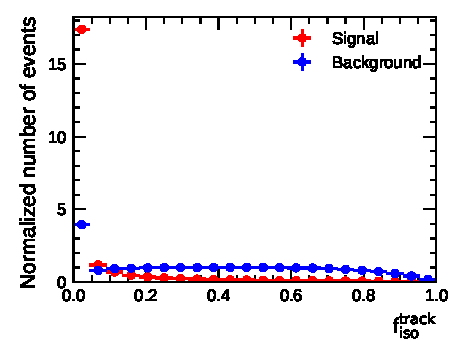
\includegraphics{./figures/baseline_bdt_vars/1p/SumPtTrkFrac.pdf}
    \subcaption{Momentum fraction of isolation tracks for 1-prong candidates.}
    \label{fig:sumpttrkfrac}
  \end{subfigure}\hfill
  \begin{subfigure}[t]{0.48\textwidth}
    \centering
    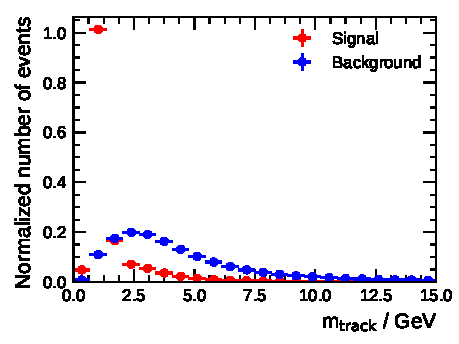
\includegraphics{./figures/baseline_bdt_vars/3p/massTrkSys.pdf}
    \subcaption{Mass of the track system for 3-prong candidates.}
    \label{fig:masstrksys}
  \end{subfigure}
  \caption{Distributions of important variables for tau identification in
    \tauhadvis candidates from simulated \mbox{$\gamma^* \to \tauhad\tauhad$}
    (signal) and dijet (background) events.}
  \label{fig:bdt_discriminants}
\end{figure}

\begin{table}[htb]
  \centering
  {\def\arraystretch{1.35}\small\begin{tabular}{ccc}
  \toprule
  Variable & 1-track & 3-track \\
  \midrule
  \smash{$f _\text{cent}$} & \textbullet & \textbullet \\
  \smash{$f_\text{leadtrack}^{-1}$} & \textbullet & \textbullet \\
  \smash{$R_\text{track}$} & \textbullet & \textbullet\\
  \smash{$\Delta R_\text{max}$} & & \textbullet \\
  \smash{$| S_\text{leadtrack} |$} & \textbullet & \\
  \smash{$S_\text{T}^\text{flight}$} & & \textbullet \\
  \bottomrule
\end{tabular}\hspace*{2em}
\begin{tabular}{ccc}
  \toprule
  Variable & 1-track & 3-track \\
  \midrule
  \smash{$f_\text{iso}^\text{track}$} & \textbullet & \\
  \smash{$f_\text{EM}^\text{track-HAD}$} & \textbullet & \textbullet \\
  \smash{$f_\text{track}^\text{EM}$} & \textbullet & \textbullet \\
  \smash{$p_\text{T}^\text{EM+track} / p_\text{T}$} & \textbullet & \textbullet \\
  \smash{$m_\text{EM+track}$} & \textbullet & \textbullet \\
  \smash{$m_\text{track}$} & & \textbullet \\
  \bottomrule
\end{tabular}

%%% Local Variables:
%%% mode: latex
%%% TeX-master: "../mythesis"
%%% End:
}
  \caption{Variables used for tau identification of \tauhadvis candidates with
    one or three reconstructed \emph{charged} tracks.}
  \label{tab:baseline_variables}
\end{table}

\subsection{BDT Configuration for Tau Identification}
In the following the initial BDT configurations employed by the tau
identification in the ATLAS reconstruction framework is summarised. At the time
of writing, the improvements presented in this chapter have been partially
implemented in the latest reconstruction release.

The training and evaluation of the tau identification BDTs is performed using
TMVA~\cite{tmva}. The initial configuration uses decision trees limited to a
maximum depth~$d_\text{tree} = 8$. The minimum fraction of training events in a
node considered for further splitting
is~$f_\text{node}^\text{min} = \SI{0.1}{\percent}$. An ensemble
of~$N_\text{trees} = 100$ decision trees is trained using the \emph{AdaBoost}
boosting algorithm with a learning rate~$\beta = 0.2$. Individual decision trees
return estimated class probabilities instead of the majority class and no
\emph{pruning} of statistically insignificant nodes is applied. This
configuration is used as a starting point for further optimisations. The full
configurations of the TMVA-BDTs are summarised in
Appendix~\ref{app:tmva_config}.

\section{Event Simulation, Preselection and Reweighting}
\label{sec:bdt_eventsim}

For training and performance evaluation of the tau identification, simulated
events at a centre-of-mass energy of~$\sqrt{s} = \SI{13}{\TeV}$ and an average
number of interactions per bunch crossing of~$\mu = \num{30}$ is used. The
signal samples use the process~$\gamma^* \to \tauhad \tauhad$, where at
generator-level leptonic decays of the tau lepton are disabled. In contrast to
the Drell--Yan process, no on- and off-shell production and interference with
the $Z$~boson is included. The reason is to create a sample with unpolarised tau
leptons, i.e. having the same number of positive and negative helicity tau
leptons, over a large range of ditau invariant masses. Polarisation biases the
angular distribution of the daughter particles in a tau decay and therefore the
kinematics, which is not desired when training general purpose algorithms.
Additionally, the ditau invariant mass spectrum is smooth and decreasing without
a large number of events close to the $Z$~mass, making it convenient for
performance studies. The background samples consist of simulated dijet events,
supplying fake \tauhadvis with transverse momenta of up to \SI{1800}{\GeV} at
tau energy scale. Both the signal and background samples are generated using
\textsc{Pythia}~8 with the A14 tune~\cite{a14_tune} and the NNPDF23LO PDF
set~\cite{NNPDF}. A complete summary of the simulated samples can be found in
Appendix~\ref{app:samples}.

A preselection is applied to reconstructed \tauhadvis in the event samples to
match typical selections applied at analysis level. Therefore, the tau
identification studies focus on candidates with visible transverse
momenta~$\pt > \SI{20}{\GeV}$. Reconstructed \tauhadvis are required to fall in
the acceptance range of the tracking system~$|\eta| < 2.5$, while rejecting
candidates in the transition region between barrel and end-cap of the
calorimeter~\mbox{$1.37 < |\eta| < 1.52$}. The number of reconstructed
\emph{charged} tracks must be either one or three. Additionally, \tauhadvis
candidates in the signal samples are matched to true taus at generator-level and
the same selections, i.e.\ transverse momentum, pseudorapidity, number of
charged hadrons in the decay, are applied at truth level. The number of tau
candidates in the samples after preselection is summarised in
Table~\ref{tab:sample_size}.

\begin{table}[htb]
  \centering
  {\small\begin{tabular}{lS[table-format=2.1]S[table-format=2.1]}
  \toprule
  & \multicolumn{2}{c}{Tau candidates / $10^6$} \\
  Sample & {1-prong} & {3-prong} \\
  \midrule
  Signal & 10.5 & 2.8 \\
  Background & 6.6 & 15.5 \\
  \bottomrule
\end{tabular}

%%% Local Variables:
%%% mode: latex
%%% TeX-master: "../mythesis"
%%% End:
}
  \caption{Number of \tauhadvis candidates after preselection.}
  \label{tab:sample_size}
\end{table}

In Figure~\ref{fig:pt_mu} the pile-up profile of the simulation and the
distribution of visible transverse momenta of \tauhadvis candidates in the
signal and background samples is shown. Since the samples are created using
different processes, their $p_\text{T}$-spectra differ. When training
identification algorithms it is important to avoid distinguishing signal and
background candidates by their transverse momentum. Therefore, weights are
applied to \tauhadvis candidates in the background sample such that the weighted
background sample is indistinguishable from the signal sample in the
reconstructed transverse momentum.

\begin{figure}[htb]
  \centering
  \begin{subfigure}[t]{0.48\textwidth}
    \centering
    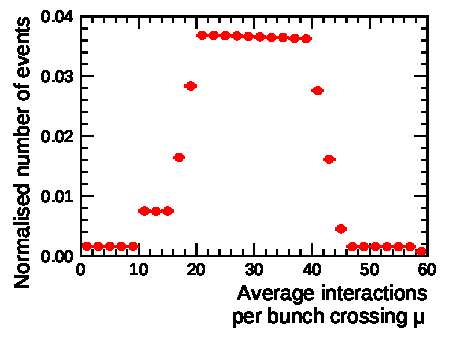
\includegraphics{./figures/bdt_perf/pt_mu_samples/mu.pdf}
    \subcaption{Pile-up profile used in the simulation.}
  \end{subfigure}\hfill
  \begin{subfigure}[t]{0.48\textwidth}
    \centering
    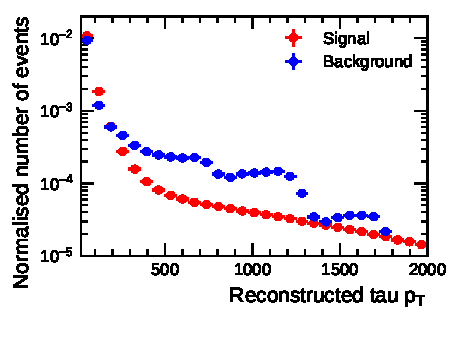
\includegraphics{./figures/bdt_perf/pt_mu_samples/pt.pdf}
    \subcaption{Transverse momentum distribution of \tauhadvis at tau energy
      scale after preselection.}
  \end{subfigure}
  \caption{Properties of the simulated signal and background samples.}
  \label{fig:pt_mu}
\end{figure}

% \todo[inline]{Reweighting, Quark-Gluon Fraction (3P: \SI{55}{\percent} excluding
%   bottom, \SI{58}{\percent} including bottom) (1P: \SI{55}{\percent} excluding
%   bottom, \SI{59}{\percent} including bottom); approx.\ \SI{60}{\percent}
%   quark-gluon fraction}


\section{Hyperparameter Optimisation}
\label{sec:bdt_hyperparam}

Machine learning algorithms typically have parameters defining the complexity of
the model. They cannot be determined as part of the training process and are
therefore called hyperparameters. Often these parameters need tuning to obtain
the best discriminative power for the underlying problem. In the following the
BDTs of the 1- and 3-prong tau identification are optimised separately with
respect to the boosting algorithm and the most important hyperparameters.

Many input variables for the identification have skewed or long-tailed
distributions leading to suboptimal decision trees as TMVA uses equidistant
sampling points for finding the best possible split on a given variable.
Therefore, transformations are applied to the variables to improve the split
finding. For this highly skewed distributions are log-transformed, while
long-tailed distributions and outliers due to detector resolution effects are
clamped to fall into a specified range of values. The exact transformations can
be found in Appendix~\ref{app:variable_transforms}.

Hold-out validation is used to measure how well the model generalises to data
that was not used to train the model. This is done by splitting the signal and
background samples into two equally sized samples called training and testing
sample. The training sample is used to train the model and the testing sample is
used to determine the performance characteristics of the model. Unless otherwise
noted, the metrics and figures given in the following sections are evaluated
using the testing sample.

\subsection{Boosting Algorithm}
\label{sec:bdt_boosting}

In Chapter~\ref{sec:ml_boosting} the two boosting algorithms \emph{AdaBoost} and
\emph{Gradient Boosting} were introduced. The performance of both algorithms for
tau identification is compared by training BDTs and varying a boosting-specific
parameter called the learning rate. The learning rate for \emph{AdaBoost} is
typically denoted by~$\beta$, while for gradient boosting it is called the
shrinkage~$\eta$. Reducing the learning rate artificially slows down the
boosting process by decreasing the influence of additional trees on the
ensemble. Empirically it has been found that small learning rates often lead to
improvements in test error~\cite{esl}.

The 1-prong tau identification BDT with the input variables and configuration
summarised in Section~\ref{sec:bdt_tauid} is trained on \tauhadvis candidates
from the signal and background samples. The learning rates for both boosting
algorithms are varied between 0.05 and 1.0. At each setting the background
rejection is calculated at a fixed signal efficiency of~\SI{60}{\percent}. For
this a single cut on the output score of the BDT is determined such
that~\SI{60}{\percent} of \tauhadvis candidates in the signal sample pass this
selection. This is an approximation of the tight working point of the tau
identification used in the ATLAS experiment. The working points will be formally
introduced at a later point.

In Figure~\ref{fig:bdt_boosting_alg} the rejection is shown as a function of the
learning rate for both algorithms. An improvement in rejection of approximately
\SI{10}{\percent} is observed when using \emph{Gradient Boosting}. The reason
for this improvement is the robust loss function (binomial log-likelihood loss)
used in the \emph{Gradient Boosting} implementation of TMVA. The loss functions
are depicted in Figure~\ref{fig:boosting_loss} showing that the \emph{Gradient
  Boosting} implementation puts less emphasis on misclassified events
($y f(x) < 0$) compared to the exponential loss of \emph{AdaBoost}. This makes
\emph{Gradient Boosting} a robust choice for problems where signal and
background are inseparable in certain regions of the input variable space. For
tau identification this can be the case for jets initiated by light quarks,
which more closely resemble hadronic decays of tau leptons. A similar
improvement is observed for the 3-prong identification, therefore \emph{Gradient
  Boosting} will be used for further optimisation steps.

\begin{figure}[htb]
  \centering
  \begin{subfigure}[t]{0.48\textwidth}
    \centering
    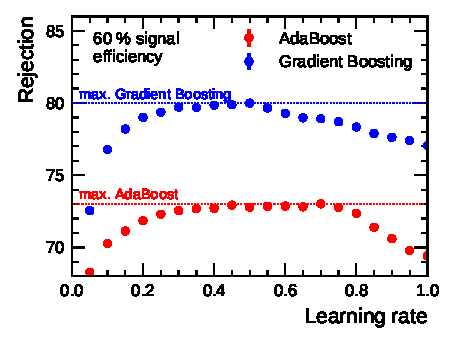
\includegraphics{./figures/bdt_perf/boosting.pdf}
    \subcaption{Rejection of 1-prong \tauhadvis candidates from dijet events
      using BDTs trained with different boosting algorithms.}
    \label{fig:bdt_boosting_alg}
  \end{subfigure}\hfill
  \begin{subfigure}[t]{0.48\textwidth}
    \centering
    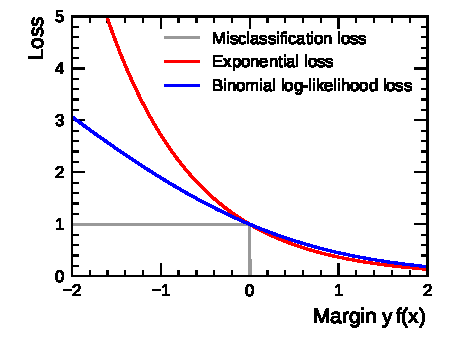
\includegraphics{./figures/theory/boosting_loss.pdf}
    \subcaption{Classification losses as a function of the margin~$y f(x)$ with
      the true class~$y \in \{-1, 1\}$ and the BDT response~$f(x) \in [-1, 1]$.
      Adapted from Ref.~\cite{esl}.}
    \label{fig:boosting_loss}
  \end{subfigure}
  \caption{Optimisation of the boosting algorithm used for tau identification.}
\end{figure}

\subsection{Grid Search in Hyperparameter Space}
\label{sec:bdt_grid_search}

Aside from the boosting algorithm, BDTs have other important hyperparameters
that need to be optimised to obtain the best possible performance. These are the
number of trees~ $N_\text{trees}$ in the ensemble and the learning rate~$\eta$.
Both parameters are boosting-specific and related as small learning rates
require a large number of trees to converge and vice versa. Additionally, the
maximum tree depth~$d_\text{tree}$ and the fraction of events required for node
splitting~$f_\text{node}^\text{min}$ are important parameters related to
individual decision trees in the ensemble. Both parameters limit the depth of a
tree and therefore the allowed order of variable interactions (e.g.\
$d_\text{tree} = 2$ allows interactions of up to two variables). The final
parameter that is investigated is \emph{bagged boosting} where each tree is
grown using a random sample of training events drawn with replacement from the
full training sample. This method aims to reduce overfitting, which is models
learning statistical fluctuations in the training sample and thus reducing
generalisation performance. The corresponding hyperparameter is the fraction of
events~$f_\text{bag}$ in the random sample.

These hyperparameters are optimised by forming a grid in the hyperparameter
space and training a BDT for each point on this grid. Subsequently, the
performance of each trained BDT is evaluated. The grid is defined by the
following hyperparameter values
\begin{align*}
  N_\mathrm{trees} &\in \{25, 50, 100, 200, 400, 800\} & \eta &\in \{0.05, 0.1, 0.2, 0.4\} & d_\mathrm{tree} &\in \{4, 6, 8, 12, 16\}\\
  f_\mathrm{node}^\mathrm{min} &\in \{\SI{0.01}{\percent}, \SI{0.1}{\percent},\SI{1.0}{\percent}\} & f_\text{bag} &\in \{\text{None}, \SI{50}{\percent} \}
\end{align*}
resulting in a total of 720 grid points each for the 1- and 3-prong BDT. The
rejection is, analogously to the previous section, calculated using a single cut
on the output score to obtain a signal efficiency comparable to the tight
working point.

In Figure~\ref{fig:hyperparameter_scan_1p} the background rejection of the
1-prong tau identification BDT is shown as a function of the hyperparameters of
the model. The relation between the hyperparameters and their impact on the
background rejection are discussed in the following.

\begin{figure}[htb]
  \begin{subfigure}[t]{0.48\textwidth}
    \centering
    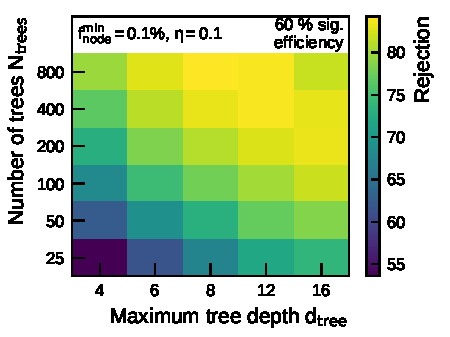
\includegraphics{./figures/bdt_perf/gridsearch_1p/scan_MaxDepth_NTrees.pdf}
    \vspace*{-1.6em}
    \subcaption{}
    \label{fig:gridscan_maxdepth_ntrees}
  \end{subfigure}\hfill
  \begin{subfigure}[t]{0.48\textwidth}
    \centering
    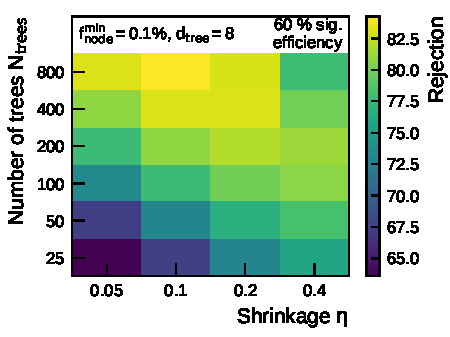
\includegraphics{./figures/bdt_perf/gridsearch_1p/scan_Shrinkage_NTrees.pdf}
    \vspace*{-1.6em}
    \subcaption{}
    \label{fig:gridscan_shrinkage_ntrees}
  \end{subfigure}
  \begin{subfigure}[t]{0.48\textwidth}
    \centering
    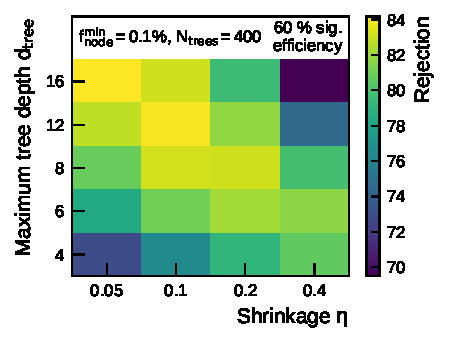
\includegraphics{./figures/bdt_perf/gridsearch_1p/scan_Shrinkage_MaxDepth.pdf}
    \vspace*{-1.6em}
    \subcaption{}
    \label{fig:gridscan_shrinkage_maxdepth}
  \end{subfigure}\hfill
  \begin{subfigure}[t]{0.48\textwidth}
    \centering
    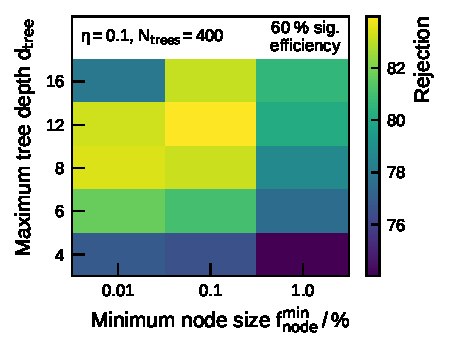
\includegraphics{./figures/bdt_perf/gridsearch_1p/scan_MinNodeSize_MaxDepth.pdf}
    \vspace*{-1.6em}
    \subcaption{}
    \label{fig:gridscan_minnodesize_maxdepth}
  \end{subfigure}
  \vspace*{-0.3em}
  \caption{Background rejection of the 1-prong BDT at \SI{60}{\percent} signal
    efficiency as a function of BDT hyperparameters. Bagged boosting with a
    sample fraction~$f_\text{bag} = \SI{50}{\percent}$ is used. The rejection is
    calculated using the testing sample.}
  \label{fig:hyperparameter_scan_1p}
\end{figure}

The interaction of the number of trees in the ensemble~$N_\text{trees}$ with the
maximum tree depth~$d_\text{tree}$ and learning rate~$\eta$ is shown in
Figures~\ref{fig:gridscan_maxdepth_ntrees} and
\subref{fig:gridscan_shrinkage_ntrees}. A distinct trade-off between the
hyperparameters~$d_\text{tree}$ and $N_\text{trees}$ can be observed , where a
large number of shallow trees and a smaller number of deep trees can reach a
similar background rejection. Moreover, small learning rates~$\eta$ require more
trees to properly fit the model. For a large number of trees and large maximum
tree depths or learning rates the model overfits leading to a reduced background
rejection in the testing sample. This effect can also be observed in
Figure~\ref{fig:gridscan_shrinkage_maxdepth}, where trees with a depth of 16 can
significantly overfit if the learning rate is set too large. The importance of
choosing an appropriate minimum node size~$f_\text{node}^\text{min}$ is shown in
Figure~\ref{fig:gridscan_minnodesize_maxdepth}. If it is chosen too large the
model does not fully capture the data. However, a small minimum node size can
quickly lead to overfitting for decision trees with large maximum depth. This is
due to the interplay of~$d_\text{tree}$ and~$f_\text{node}^\text{min}$, when
constraining the depth of the decision trees. The optimisation of the 3-prong
tau identification shows similar results, which are summarised in
Appendix~\ref{app:grid_search_3p} and are omitted here for brevity.

Table~\ref{tab:bdt_perfs} summarises two configuration for the 1- and 3-prong
BDT. The models denoted by \mbox{BDT A} consist of the BDTs with the largest
rejection at the corresponding signal efficiency. One observes that these
configurations fall on the edge of the parameter grid, indicating that a
configuration with larger rejection could be found outside of the scanned
hyperparameter region. However, the distributions of the BDT scores for signal
and background \tauhadvis candidates on both the training and testing sample in
Figure~\ref{fig:bdt_score_1p} show a significant deviation between training and
testing sample. This is due to the model learning statistical fluctuations in
the training sample which are not present in the testing sample, indicating that
the models are close to overfitting. These deviations are most significant for
the 1-prong background and the 3-prong signal distributions due to their limited
sample size (cf.\ Table~\ref{tab:sample_size}).

% The one-prong BDT is optimised for efficiency of the tight working-point (in the
% scan no flattening was applied). However the 3-prong BDT was optimised for the
% loose working-point, because the rejection of the 3-prong ID is roughly one
% order of magnitude larger thus the tight working-point is not a stable metric
% considering the size of the available background sample.

\begin{table}[htb]
  \centering
  {\small\begin{tabular}{ll
  S[table-format=3.0]
  S[table-format=1.2]
  S[table-format=2.0]
  S[table-format=1.2]
  c}
  \toprule
  & Name & {$N_\text{trees}$} & {$\eta$} & {$d_\text{tree}$} & {$f_\text{node}^\text{min}$ / \si{\percent}} & {$f_\text{bag}$} \\
  \midrule
  \multirow{2}{*}{1-prong} & BDT A & 800 & 0.05 & 16 & 0.01 & -- \\
  & BDT B & 400 & 0.1 & 8 & 0.1 & \SI{50}{\percent} \\
  \midrule
  \multirow{2}{*}{3-prong} & BDT A & 800 & 0.1 & 16 & 0.01 & -- \\
  & BDT B & 800 & 0.4 & 6 & 0.1 & -- \\
  \bottomrule
\end{tabular}

%%% Local Variables:
%%% mode: latex
%%% TeX-master: "../mythesis"
%%% End:
}
  \caption{BDT configurations after systematic optimisation. BDT~A denotes the
    BDT with the largest rejection on the testing sample, while BDT~B also
    requires a KS test $p$-value of at least \SI{5}{\percent} for compatibility
    of the BDT score distributions on training and testing sample. The rejection
    is given at \SI{60}{\percent} (\SI{45}{\percent}) signal efficiency for the
    1-prong (3-prong) identification.}
  \label{tab:bdt_perfs}
\end{table}

\begin{figure}[htb]
  \begin{subfigure}[t]{0.48\textwidth}
    \centering
    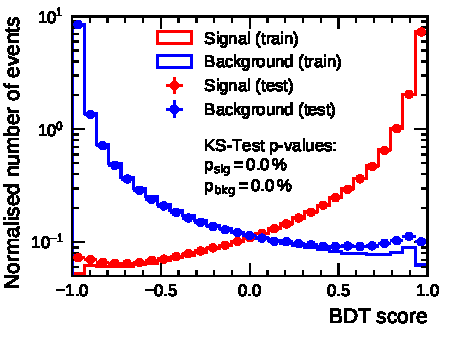
\includegraphics{./figures/bdt_perf/scores/grid_1p0304.pdf}
    \subcaption{BDT A}
    \label{fig:bdt_score_1p}
  \end{subfigure}\hfill
  \begin{subfigure}[t]{0.48\textwidth}
    \centering
    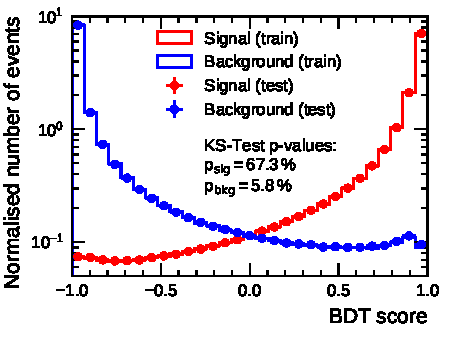
\includegraphics{./figures/bdt_perf/scores/grid_1p_subsampling0269.pdf}
    \subcaption{BDT B}
    \label{fig:bdt_score_1p_ks5}
  \end{subfigure}
  \caption{Distributions of the 1-prong tau identification BDT score for the
    training and testing sample for signal and background candidates.}
  \label{fig:bdt_overfitting_scores}
\end{figure}

Instead of choosing the BDT with the largest rejection, compatibility of the BDT
score distributions in the training and testing sample is also required. This is
done to improve the robustness to a potential decrease in training statistics
for future trainings of the tau identification. The compatibility of two
distributions is measured using the $p$-value of the Kolmogorov--Smirnov test
(KS test). The configuration~\mbox{BDT B} in Table~\ref{tab:bdt_perfs} consists
of the BDT with the highest rejection at the specified signal efficiency, while
also requiring that the $p$-value of the KS test between training and testing
sample is larger than \SI{5}{\percent}. The score distributions after requiring
compatibility according to the KS test is shown in
Figure~\ref{fig:bdt_score_1p_ks5}. For completeness the distributions for the
3-prong case are summarised in Appendix~\ref{app:bdt_stuff}.

The operating point of a BDT depends on the threshold applied to its output
score, thus defining a trade-off between signal efficiency and background
rejection. Figure~\ref{fig:bdt_rocs} shows the performance characteristics as
the classification threshold is varied and is called the receiver operating
characteristic curve (ROC-curve). Comparing \mbox{BDT A} and \mbox{BDT B} for
the 1- and 3-prong identification, the decrease in rejection of the conservative
model is less than \SI{5}{\percent} over the relevant efficiency range.
Moreover, the rejection of the conservative \mbox{BDT B} improves on the
reference by \num{10} to \SI{16}{\percent}. The rejection of the 3-prong BDT is
approximately one order of magnitude larger than for the 1-prong case. This can
largely be attributed to the availablility of invariant mass and secondary
vertex information.

\begin{figure}[htb]
  \begin{subfigure}[t]{0.48\textwidth}
    \centering
    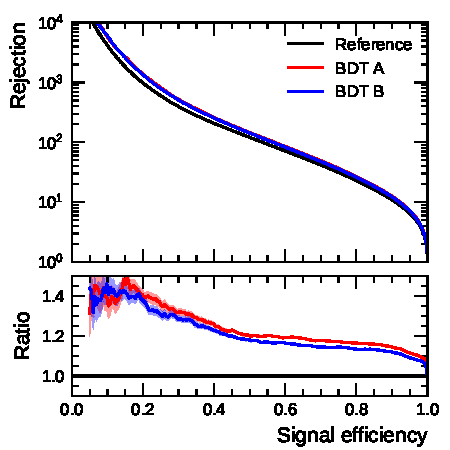
\includegraphics{./figures/bdt_perf/roc/bootstrap_roc_comparison_1p.pdf}
    \subcaption{1-prong}
    \label{fig:bdt_1p_roc}
  \end{subfigure}\hfill
  \begin{subfigure}[t]{0.48\textwidth}
    \centering
    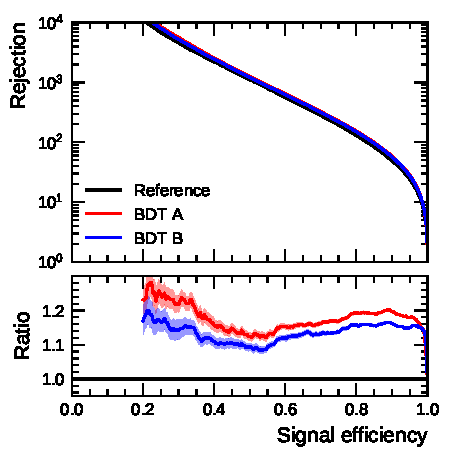
\includegraphics{./figures/bdt_perf/roc/bootstrap_roc_comparison_3p.pdf}
    \subcaption{3-prong}
    \label{fig:bdt_3p_roc}
  \end{subfigure}
  \caption{ROC-Curves for BDT A, BDT B and a comparison with the reference
    configuration. The ratio of the rejection with respect to the reference is
    depicted in the lower panel.}
  \label{fig:bdt_rocs}
\end{figure}

\section{Tau Identification Working Points}
\label{sec:bdt_working_points}

For the use of tau identification in analyses, four working points with fixed
signal efficiencies are defined. The efficiencies of the working points are
given in Table~\ref{tab:wp_eff}. Due to the abundance of 3-track \tauhadvis
candidates originating from multijet events, a tighter selection is applied to
the 3-prong tau identification.

\begin{table}[htb]
  \centering
  {\small\begin{tabular}{lcc}
  \toprule
  & \multicolumn{2}{c}{Signal efficiency} \\
  Working point & 1-prong & 3-prong \\
  \midrule
  Very Loose & 95\% & 95\% \\
  Loose & 85\% & 75\% \\
  Medium & 75\% & 60\% \\
  Tight & 60\% & 45\% \\
  \bottomrule
\end{tabular}

%%% Local Variables:
%%% mode: latex
%%% TeX-master: "../mythesis"
%%% End:
}
  \caption{Efficiencies of the tau identification working points.}
  \label{tab:wp_eff}
\end{table}

The decision threshold of the BDT is parametrised as a function of the
reconstructed transverse momentum of the \tauhadvis candidate at the tau energy
scale and the average number of interactions per bunch crossing~$\mu$. This is
done to ensure a constant signal efficiency over a wide transverse momentum
range and in different pile-up scenarios. The average number of interactions per
bunch crossing is used instead of the number of reconstructed primary vertices
to ensure compatibility with the identification at the tau trigger, where track
and vertex information is unavailable due time constraints.

The thresholds on the BDT score are calculated in bins
of~\tauhadvis~$p_\text{T}$ and~$\mu$, such that the signal efficiency in each
bin reaches the target efficiency of the working point. In
Figure~\ref{fig:working_point_cutmap} the threshold maps are depicted for the
tight working point of the 1- and 3-prong identification using the conservative
\mbox{BDT B}. The binning is chosen such that the derived thresholds are not
dominated by statistical fluctuations due to the limited number of events in
certain bins (cf.\ pile-up profile and \tauhadvis $p_\text{T}$-spectrum in
Figure~\ref{fig:pt_mu}).

\begin{figure}[htb]
  \centering
  \begin{subfigure}[t]{0.48\textwidth}
    \centering
    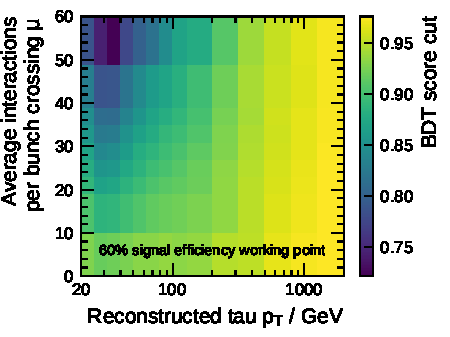
\includegraphics{./figures/bdt_perf/working_points/grid_1p_subsampling0269_wp.pdf}
    \subcaption{1-prong}
  \end{subfigure}\hfill
  \begin{subfigure}[t]{0.48\textwidth}
    \centering
    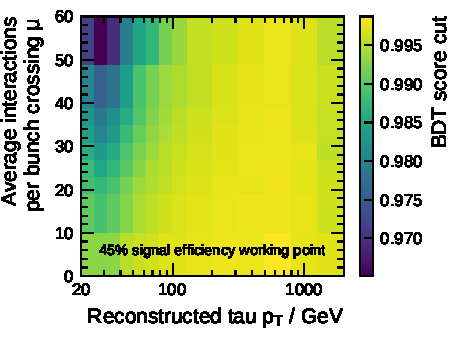
\includegraphics{./figures/bdt_perf/working_points/grid_3p0327_wp.pdf}
    \subcaption{3-prong}
  \end{subfigure}
  \caption{Decision thresholds for the tight working point using \mbox{BDT B}.}
  \label{fig:working_point_cutmap}
\end{figure}

The behaviour of the thresholds with respect to the visible transverse momentum
of \tauhadvis and the average number of interactions per bunch crossing is
similar for the 1- and 3-prong identification. The thresholds tend to get larger
(tighter) with increasing transverse momentum. This is due to the boost of the
tau lepton leading to larger decay lengths and more collimated daughter
particles, thus making the decay more tau-like. At low transverse momenta and
high pile-up the thresholds are looser due to pile-up widening the signature of
the decay in the calorimeter. Finally, the dependency of the thresholds on the
amount of pile-up decreases for large transverse momenta, as the soft pile-up
cannot significantly alter the signature of the highly energetic tau decay.

\section{Variable Selection}
\label{sec:bdt_variable_selection}

After optimising the hyperparameter configuration and defining the working
points to be used by analyses, an investigation of the input variable selection
is performed. First the set of variables is extended to improve the rejection of
\tauhadvis candidates from quark- or gluon-initiated jets. Subsequently, input
variables with an insignificant impact on the discriminative power are removed
to simplify the model.

\subsection{Transverse Momentum Dependency of the Input Variables}
\label{sec:bdt_incl_pt}

% Do I need these plots?
% \begin{figure}[ht]
%   \begin{subfigure}[t]{0.48\textwidth}
%     \centering
%     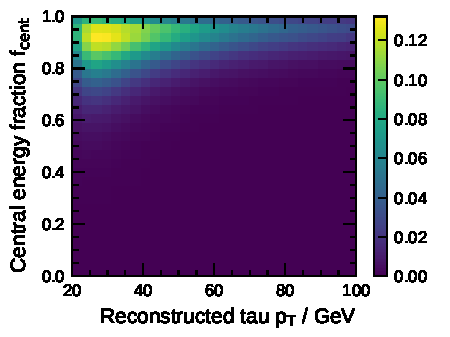
\includegraphics{./figures/bdt_perf/cent_frac_vs_pt_sig.pdf}
%     \subcaption{Signal}
%   \end{subfigure}\hfill
%   \begin{subfigure}[t]{0.48\textwidth}
%     \centering
%     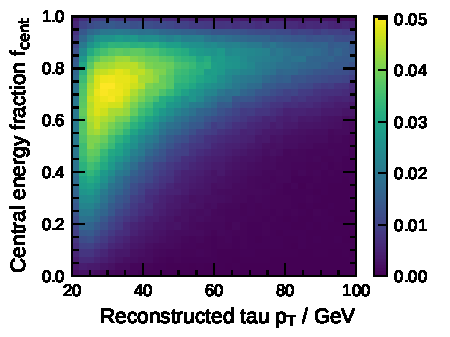
\includegraphics{./figures/bdt_perf/cent_frac_vs_pt_bkg.pdf}
%     \subcaption{Background}
%   \end{subfigure}
%     \caption{$p_\text{T}$-dependency of the central energy fraction.}
%   \label{fig:bdt_pt_dependency}
% \end{figure}

The distributions of the variables used for tau identification change depending
on the reconstructed transverse momentum of the \tauhadvis candidates. This
impacts the identification algorithm as the separation of signal and background
in a given variable varies as a function of~$p_\text{T}$.

Variables that are affected by this are the track radius~$R_\text{track}$ and
the maximum track~$\Delta R$. At large transverse momentum \emph{charged} tracks
tend to be closer to the tau axis for both signal and background candidates,
thus reducing the separation in these variables. Similarly, the central energy
fraction~$f_\text{cent}$ of background candidates increases at high transverse
momentum making them more tau-like. In contrast to this, the variables based on
invariant masses~$m_\text{track}$ and~$m_\text{EM+track}$ show a larger
separation at high transverse momentum. This is because the mass of signal
candidates is bounded by the mass of the tau lepton, while for candidates from
quark- or gluon-initiated jets the invariant mass tends to increase with
increasing transverse momentum of the \tauhadvis candidate. \todo{Plots?
  Actually not true...}

To take advantage of the varying signal/background separation in different
$p_\text{T}$-regions, the \tauhadvis transverse momentum is included as an input
to the BDT. Correlations between the remaining input variables and \tauhadvis
\pt can then be used to distinguish signal and background candidates. The
kinematic reweighting (cf.\ Section~\ref{sec:bdt_eventsim}) ensures that the
classification only uses correlations of the transverse momentum with the
remaining inputs and not the distinct $p_\text{T}$-spectra of the signal and
background samples.

For the use of tau identification in analyses, the working point efficiencies in
data must be determined in a tag-and-probe measurement. Due to the limited
number of \tauhadvis with transverse momenta greater than \SI{100}{\GeV}, the
efficiency measurement needs to extrapolate to higher $p_\text{T}$-regions.
Therefore, it should be avoided to introduce an explicit $p_\text{T}$-dependence
for transverse momenta larger than \SI{100}{\GeV} into the BDTs. This is
realised by \emph{clamping} the transverse momentum
\begin{align*}
  p_\text{T}^\text{clamp} = \min(p_\text{T}, \SI{100}{\giga\electronvolt})
\end{align*}
for the use in the BDT. An implicit dependency cannot be avoided due to the
correlations of the remaining identification variables with the reconstructed
transverse momentum.

The \emph{clamped} transverse momentum at LC scale is included as an input
variable into the BDT. No tau-specific energy calibration is used to avoid
introducing systematic errors due to the calibration. Moreover, the
discriminative power of the identification does not benefit from using the tau
energy scale calibration. In Table~\ref{tab:bdt_new_variables} the relative
rejection gain is summarised after including the transverse momentum. Including
the clamped momentum~\smash{$p_\text{T}^\text{clamp}$} increases the average
rejection by up to \SI{4.9 +- 0.2}{\percent} for the 1-prong loose, and \SI{3.6
  +- 0.5}{\percent} for the 3-prong medium working point. The comparison of the
relative rejection gain after including the unclamped momentum~$p_\text{T}$ and
the clamped momentum~\smash{$p_\text{T}^\text{clamp}$} show that the majority of
rejection is retained after clamping.

Also shown in the table is the rejection after including the momentum fraction
of isolation tracks~$f_\text{iso}^\text{track}$ into the 3-prong BDT, where it
was previously not used. It shows a significant improvement in rejection
especially at the loose and medium working points.

\begin{table}[htb]
  \centering
  {\small\begin{tabular}{
  l
  p{1.5cm}
  S[table-format=1.1(1)]
  S[table-format=1.1(1)]
  S[table-format=1.1(1)]
  }
  \toprule
  & \multirow{2}{*}[-0.15em]{Variable} & \multicolumn{3}{c}{relative rejection gain / \si{\percent}} \\
  \cmidrule{3-5}
  & & {tight} & {medium} & {loose}\\
  \midrule
  \multirow{2}{*}{\vspace*{-0.2em}1-prong} & $p_\text{T}$ & 4.3 +- 0.4 & 4.4 +- 0.3 & 5.6 +- 0.2 \\[0.2em]
  & $p_\text{T}^\text{clamp}$ & 3.5 +- 0.3 & 3.8 +- 0.3 & 4.9 +- 0.2 \\
  \midrule
  \multirow{3}{*}{\vspace*{-0.4em}3-prong} & $p_\text{T}$ & 2.7 +- 0.9 & 3.9 +- 0.6 & 3.1 +- 0.3 \\[0.2em]
  & $p_\text{T}^\text{clamp}$ & 2.3 +- 0.9 & 3.6 +- 0.5 & 3.1 +- 0.3 \\[0.2em]
  & $f_\text{iso}^\text{track}$ & 3.0 +- 1.0 & 5.6 +- 0.6 & 6.6 +- 0.5 \\
  \bottomrule
\end{tabular}

%%% Local Variables:
%%% mode: latex
%%% TeX-master: "../mythesis"
%%% End:
}
  \caption{Relative gain in background rejection after including additional
    variables.}
  \label{tab:bdt_new_variables}
\end{table}

\subsection{Variable Importance}
\label{sec:bdt_var_importance}

After including the transverse momentum~\smash{$p_\text{T}^\text{clamp}$} and
the momentum fraction of isolation tracks~\smash{$f_\text{iso}^\text{track}$} as
inputs to the model, a systematic evaluation of the variable importance is
performed. The aim is to simplify the model by removing variables with small
contributions to the classification power.

The importance of individual variables is determined by training a model without
including the variable and calculating the rejection loss with respect to the
baseline model using the full variable set. Doing this for all input variables
allows to rank their importance for discriminating signal and background
\tauhadvis candidates. This method is used, as opposed to the built-in methods
of TMVA, as it properly treats correlated variables.

Figure~\ref{fig:variable_importance} depicts the variable importance for the 1-
and 3-prong BDT. The rejection loss is calculated at the tight working point for
the 1-prong and at the medium working point for the 3-prong BDT. The medium
working point is chosen due to the large rejection of the 3-prong identification
leading to less stable rankings.

\begin{figure}[htb]
  \centering
  \begin{subfigure}[t]{0.48\textwidth}
    \centering
    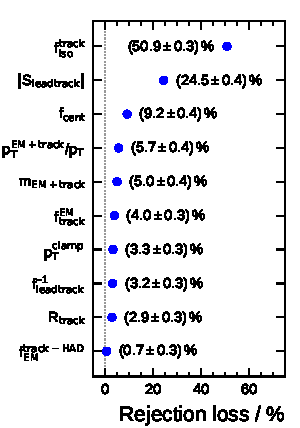
\includegraphics{./figures/bdt_perf/var_importance/1p_iter1.pdf}
    \subcaption{1-prong BDT at the tight working point with
      \SI{60}{\percent}~signal efficiency.}
  \end{subfigure}\hfill
  \begin{subfigure}[t]{0.48\textwidth}
    \centering
    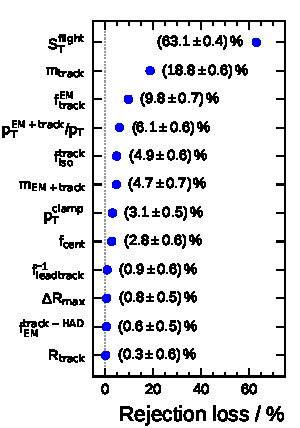
\includegraphics{./figures/bdt_perf/var_importance/3p_iter1.pdf}
    \subcaption{3-prong BDT at the medium working point with \SI{60}{\percent}
      signal efficiency.}
  \end{subfigure}
  \caption{Variable importance in the 1- and 3-prong BDT. The average rejection
    loss at the specified working point is evaluated on the weighted background
    sample and is calculated with respect to the full variable set. }
  \label{fig:variable_importance}
\end{figure}

The ranking shows that variables sensitive to the decay length of the tau
lepton, i.e.\ the transverse impact parameter
significance~$|S_\text{leadtrack}|$ and transverse flight path
significance~$S_\text{T}^\text{flight}$, have a large impact on the
classification performance. Moreover, the momentum fraction of isolation
tracks~$f_\text{iso}^\text{track}$ accounts for the majority of the background
rejection in the 1-prong identification. In the 3-prong BDT the mass of the
track system~$m_\text{track}$ contributes substantially.

The variable importance ranking identifies several weak variables used in the
BDTs. The EM energy fraction of charged
pions~\smash{$f_\text{EM}^\text{track-HAD}$} shows a small significance with a
rejection loss of~\SI{0.7 +- 0.3}{\percent} after removing it from the 1-prong
BDT. This is due to its high correlation
with~\smash{$p_\text{T}^\text{EM+track} / p_\text{T}$} with a linear correlation
coefficient of approximately \SI{70}{\percent} for both signal and background
\tauhadvis candidates. Similarly, the track radius~$R_\text{track}$ in the
3-prong BDT is highly correlated with the maximum track~$\Delta R$ and therefore
removing this variable does not result in a significant decrease in background
rejection.

After removing the first variable from each BDT the variable importance is
reevaluated to account for correlations between variables. After
removing~\smash{$f_\text{EM}^\text{track-HAD}$} from the 1-prong BDT, the
weakest variable is the track radius~$R_\text{track}$. Removing~$R_\text{track}$
leads to a rejection loss of \SI{3.2 +- 0.4}{\percent} with respect to the model
using the full variable set and is therefore kept. Following the same procedure
for the 3-prong BDT shows that~\smash{$f_\text{EM}^\text{track-HAD}$}
contributes little to the discriminative power with a rejection loss of \SI{1.2
  +- 0.6}{\percent} after removing the variable.

The set of variables and their importance after removing weak variables is
summarised in Figure~\ref{fig:variable_importance_final}. The change in input
variables alters the importance ranking slightly, especially affecting variables
that are correlated with variables that were removed (e.g.\
\smash{$p_\text{T}^\text{EM+track} / p_\text{T}$}).

\begin{figure}[htb]
  \centering
  \begin{subfigure}[t]{0.48\textwidth}
    \centering
    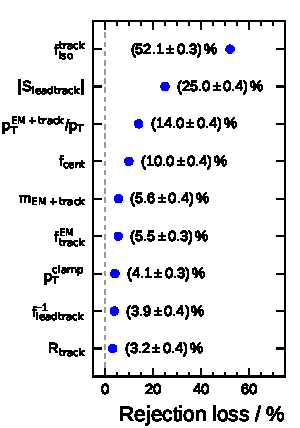
\includegraphics{./figures/bdt_perf/var_importance/1p_iter2.pdf}
    \subcaption{1-prong BDT at the tight working point with
      \SI{60}{\percent}~signal efficiency.}
  \end{subfigure}\hfill
  \begin{subfigure}[t]{0.48\textwidth}
    \centering
    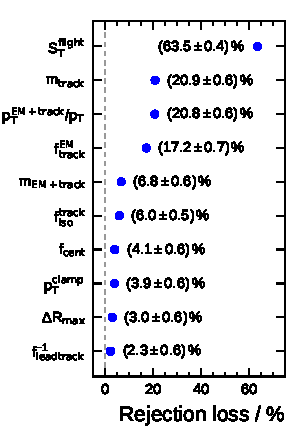
\includegraphics{./figures/bdt_perf/var_importance/3p_iter3.pdf}
    \subcaption{3-prong BDT at the medium working point with
      \SI{60}{\percent}~signal efficiency).}
  \end{subfigure}
  \caption{Variable importance in the 1- and 3-prong BDTs after removing weak
    variables. The average rejection loss at the specified working point is
    evaluated on the weighted background sample and is calculated with respect
    to the full variable set.}
  \label{fig:variable_importance_final}
\end{figure}

% Correlations:
% 1P: ChPiEMEOverCaloEME and ptRatioEflowApprox: sig (bkg) \SI{72}{\percent} (\SI{68}{\percent})
% Other large correlations: etOverPtLeadTrk and EMPOverTrkSysP \SI{86}{\percent} (\SI{90}{\percent})

% 3P: dRmax and innerTrkAvgDist correlation: sig (bkg) \SI{74}{\percent} (\SI{80}{\percent})
% 3P: ChPiEMEOverCaloEME and ptRatioEflowApprox: sig (bkg) \SI{75}{\percent} (\SI{81}{\percent})
% Other large correlations: EMPOverTrkSysP and etOverPtLeadTrk \SI{52}{\percent} (\SI{79}{\percent})

\section{Tau Identification Performance after Optimisation}
\label{sec:bdt_perf}
The performance of the optimised BDT configuration and variable selection is
subsequently evaluated on simulated data and compared with the reference BDTs
before optimisation. The optimisations include the conservative BDT
configurations (BDT B) and the revised variable selection.

Figure~\ref{fig:rejection_comparison} shows the background rejection of the 1-
and 3-prong BDT at the tight working point. After optimisation the 1-prong BDT
shows an improvement in background rejection of \num{10} to \SI{30}{\percent}
depending on the transverse momentum of the \tauhadvis candidate. \todo{Why
  large rejection at \SI{20}{\GeV}}


Similarly, the rejection at the tight working point of the 3-prong BDT also
improves on the reference by \num{10} to \SI{30}{\percent} depending on the
transverse momentum.

The medium working point shows a similar behaviour with a small improvement at
low transverse momentum.

However, the loose working point shows significant improvements exceeding
\SI{30}{\percent} with respect to the reference at
low~$p_\text{T} < \SI{25}{\GeV}$ and high transverse
momentum~$p_\text{T} > \SI{80}{\GeV}$.

In the intermediate momentum range the improvements range from \num{15} to
\SI{25}{\percent}.




For
completeness the rejection of the loose and medium working points are summarised
in Appendix~\ref{app:bdt_working_point_rejection} but show no difference
compared to the tight working point.

\begin{figure}[htbp]
  \centering
  \begin{subfigure}[t]{0.48\textwidth}
    \centering
    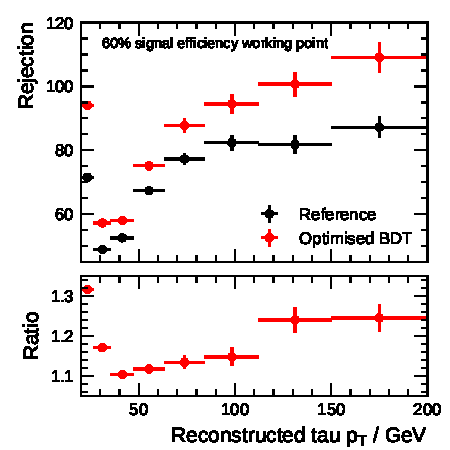
\includegraphics{./figures/bdt_perf/post_optimisation/rejection_tight_1p.pdf}
    \subcaption{1-prong}
  \end{subfigure}\hfill
  \begin{subfigure}[t]{0.48\textwidth}
    \centering
    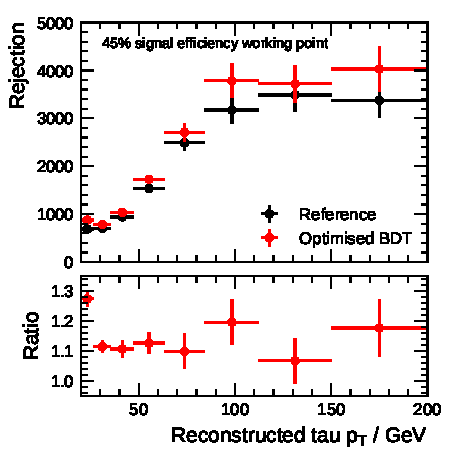
\includegraphics{./figures/bdt_perf/post_optimisation/rejection_tight_3p.pdf}
    \subcaption{3-prong}
  \end{subfigure}
  \caption{Background rejection of the tight working point as a function of
    \tauhadvis~$p_\text{T}$ at tau energy scale.}
  \label{fig:rejection_comparison}
\end{figure}


\todo[inline]{Conclusion}

% 1-prong: Gluon dominated at low pt -- 20 percent quark to gluon ratio sub 25 GeV
% 3-prong:

\todo[inline]{Working point efficiencies for pt and mu\\
  Rejection for full pt range;\\
  Plot 2nd order effects? (e.g.\ ptRatioEflowApprox vs.\ mEflowApprox 1p
  or massTrkSys vs.\ EMPOverTrkSysP 3p); \\
  Understand the rejection vs.\ pt curve. Why does the rejection drop (is it
  because rejection is enhanced due to pile-up fakes)? Why does rejection
  increase again for high pt?; \\
  BDT is optimised for a 'gammatautau'-like spectrum (focused on improving
  rejection at low pt);\\
  Show 2D plot of signal \& background e.g. massTrkSys vs. EMPOverTrkSysP to
  motivate the use of MVA methods / BDTs}

%%% Local Variables:
%%% mode: latex
%%% TeX-master: "mythesis"
%%% End:
